%\todo{RONALD - first draft by 30/May}

The \emph{Peer Manager (PM)} is a fundamental building block of the SmartSociety platform, providing a user-centered data store that maintains and manages information about human- or machine-based peers in a privacy-preserving framework. 

\subsection{Mechanisms and algorithms}
%\todo{Peer Manager Theory - including flow diagram, pseudo-code if needed, whatever explain how it works}

The PM was design as an extension of existing identity management systems to keep the information owned by peers private.
For enhancing management of information, the PM builds upon the notion of an \emph{entity-centric semantic enhanced model} that defines extensible set of entity schemas providing the templates for an attribute-based representation of peers' characteristics~\cite{Giunchiglia_fromknowledge}. Additionally, the PM defines a \emph{storage and privacy protection model} by adding privacy regulations and considerations~\cite{Hartswood:2015fe}. 
The design of this model pays special attention to different privacy issues discussed by the Council of Europe in its recommendation {\sc{cm}}/{\sc{rec}}(2010)13 on profiling \cite{CoE2010}, as well as 
basic legal privacy principles enacted by the {\sc{eu}} Data Protection Directive 95/46/{\sc{ec}} \cite{EUDir95} and that affects profiles when they involve storage and processing of personal data.

An important feature of the PM's model is that the concrete meaning of schemas is further specified by mapping single elements (i.e., types of entities, the names of attributes and their values) to concepts from an underlying ontology that is also part of the same model~\cite{Giunchiglia_fromknowledge}. Thus, allowing reasoning over peer's properties as well as the implementation of semantic-enhanced services.
%
Then the basic set of schemas/templates can be easily extended to support new application-specific scenarios requiring, for instance, the creation of new types of peers. The adaptability is provided by enabling the search and information sharing services to work over the new types in a way that is transparent to the rest of the HDA-CAS platform.

%%% Privacy%%%
Other important feature of the PM is that the privacy of peers is protected by allowing people (i.e. users) to define profiles that contain and reveal only partial or (semantically) obfuscated information that are used for replying to information requests and is thus enforcing data minimisation. 
This allows, for example, a human peer to reveal whether it is a smoker and its age range (as a way to obfuscate the age and date of birth) when participating in a ride-sharing collective, while the same information can be hidden (i.e., completely obfuscated) when participating in a question-answering collective.

%%% Architecture %%%
The details about the internal architecture of the PM was presented in~\cite{D4.2,Hartswood:2015fe}, however, we recall one of its main component (i.e., the Peer Base) in the conceptual view shown in Figure~\ref{fig:peerManagerPlatform}. It is composed of the following sub-components: 
\begin{itemize}
\item A \emph{Platform-Wide Knowledge Base} (${KB}_{PW}$) that stores the core entity types and underline ontology allowing all SmartSociety components to interoperate. 
\item A \emph{Platform-Wide Entity Base} (${EB}_{PW}$) that stores entity instances of general interests as well as public profiles of peers (i.e., information that each peer decides to publish in the platform about themselves).
\item A \emph{Knowledge Base} (${KB}_i$) and an \emph{Entity Base} (${EB}_i$) for each peer, which store the peer’s information. The peer maintains control over its data space and defines the privacy policies that apply to the data stored in it. 
%The peer's $KB$ is bootstrapped with the content of the platform-wide's $KB$, which then can be extended/specialized by the peer. The peer's $EB$ stores entity instances that are relevant to the peer (i.e., peer’s personal information, its resources, locations, roles, tasks, etc.). 
\end{itemize}
This storage separation for each of the peers and the platform is one of the Privacy-by-design decisions made by the PM in accordance to its privacy protection model.
%

\begin{figure}[t]
	\centering
	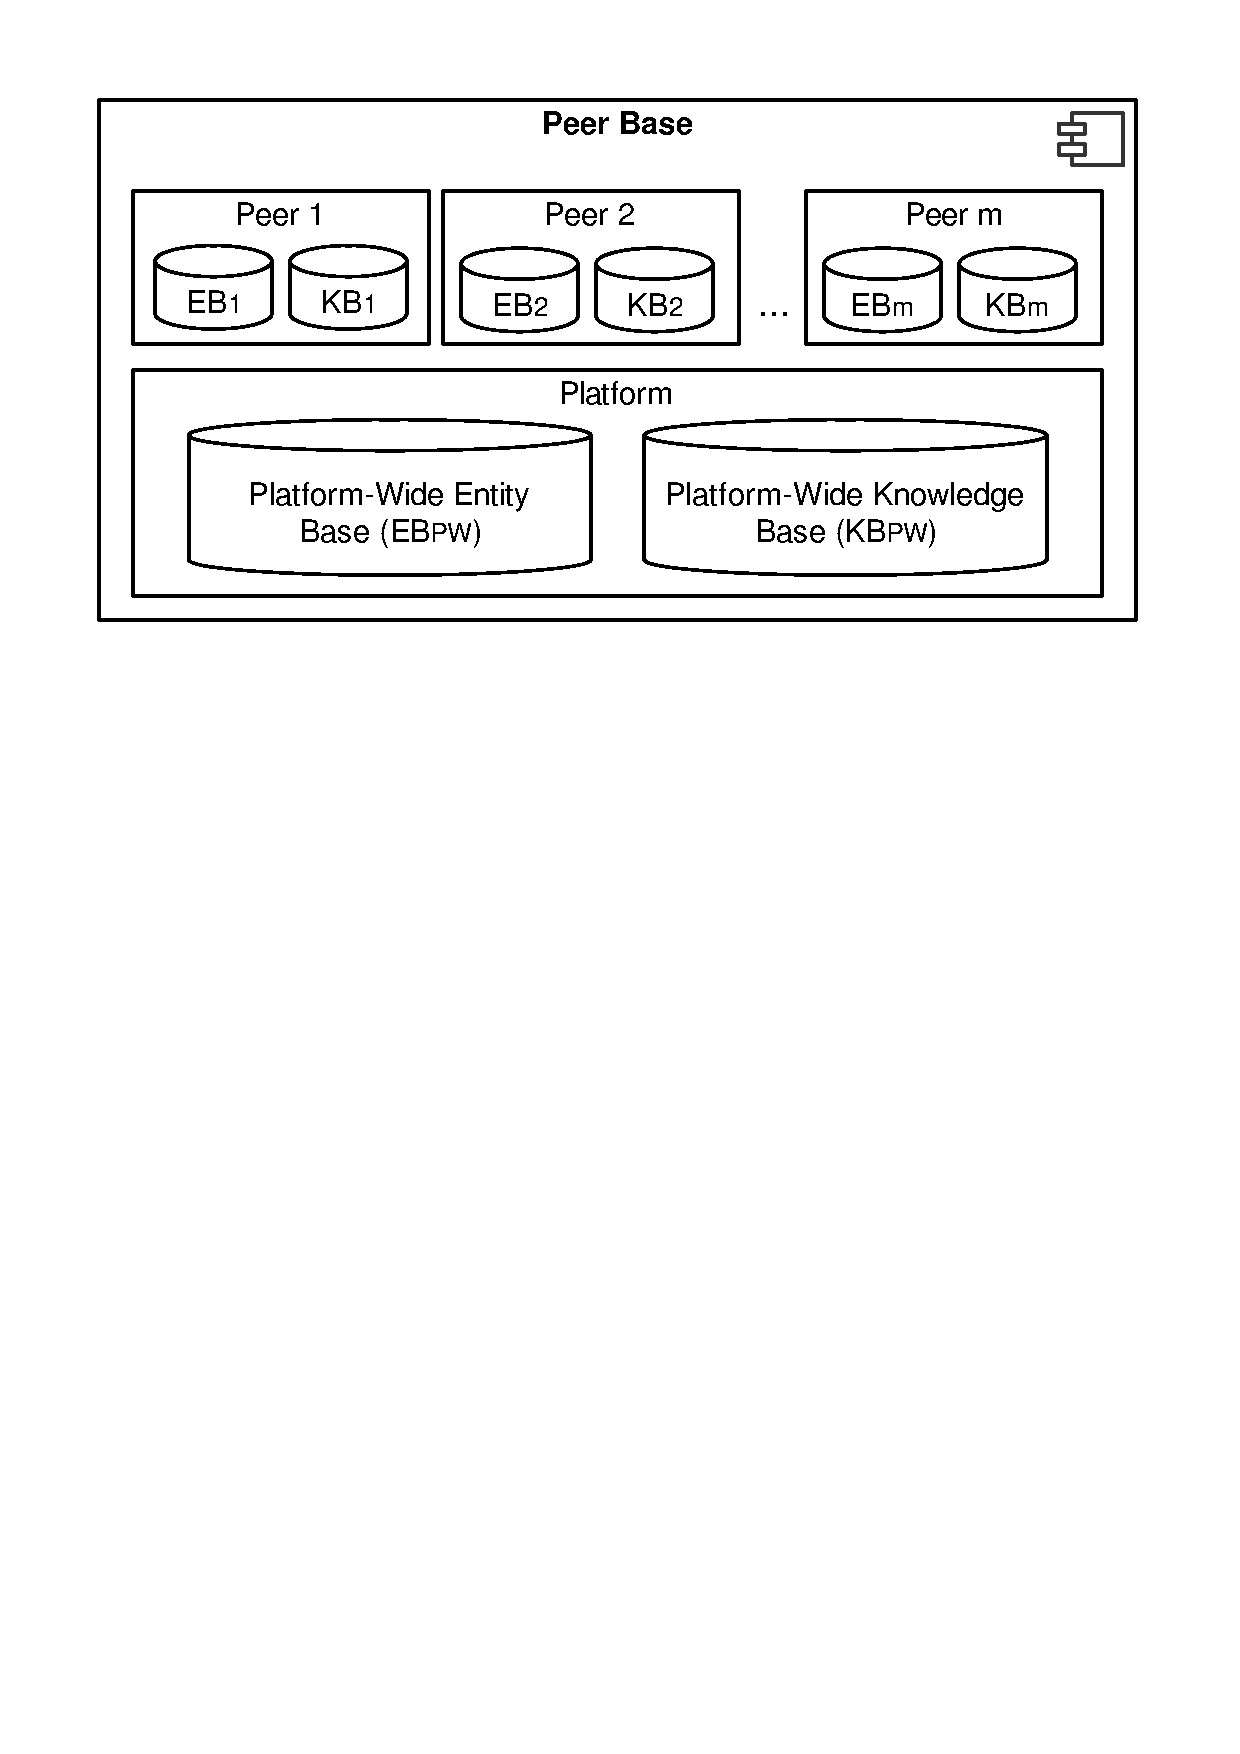
\includegraphics[width=0.7\linewidth]{figures/peerBase-diagram.pdf}
	\caption{Partial view of the Peer Manager internal architecture. Each subject its assigned its own peer storage, while the platform itself offers a shared Knowledge and Entity storages for different interactions.}
	\label{fig:peerManagerPlatform}
\end{figure}




\subsection{Implementation}
%{\it including how it has been implemented and specifications of APIs}

The Peer Manager component has been developed by following a three layered approach, where each layer leverages the basic services offered by the level below and composes them for producing higher-level services. This structure is shown in Figure~\ref{fig:pm-component-layers} and each layer will be further described in the rest of this section. 

\begin{figure}[htbp]
\centering
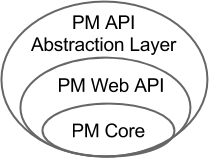
\includegraphics[width=0.4\textwidth]{figures/pm-component-layers.png}
\caption{Implementation layers of the Peer Manager}
\label{fig:pm-component-layers}
\end{figure}


\subsubsection{Peer Manager Core}
Its main purpose is to provide a privacy aware semantic storage for the SmartSociety Platform. This layer is implemented using Java, along with common data access frameworks like Spring and Hibernate.
While these technologies represent previous work from the University of Trento, the SmartSociety (through the work documented in D1.1, D4.1 and D4.2) has created the Knowledge Model used for representing peers, users, profiles (i.e. personal information) and more generally managing the information for running an HDA-CAS.

No major changes have been done to the models or structures of the Peer Manager during the first half of year three (so the research reported in previous deliverables still holds) but efforts to update these models to its final version for the SmartSociety project will start on the second part of year three (as T1.4 restarts) and will have its results reported in D1.3. It is not expected that radical changes to the models and structures are done in this revision so the underlying code and the exposes calls would probably receive only minor revisions as a result of this. 

\subsubsection{Peer Manager Web API} \label{ssec:pm-web-api}
This layer takes the Java classes that implement the Peer Manager Core and wraps them in HTTP API calls. 
No great changes, save for small adjustments and bug fixes were introduced to this layer in year three. As such the same information from deliverable D4.2 largely applies to this layer.
API specification for this layer may be found in the Appendix~\ref{sec:pm-web-api-detail}.

\todo{Content describing the purpose of this layer and the technologies used to implement it will be added to this section for the final version of this document}

\subsubsection{Peer Manager abstraction layer API} \label{ssec:pm-abs-api}
This is a new component being developed specifically for the SmartSociety project and as such all code belonging to this layer will be open sourced. API Specifications for this layer may be found in the Appendix~\ref{sec:pm-abs-api-detail}.

\todo{Content describing the purpose of this layer and the technologies used to implement it will be added to this section for the final version of this document}

\subsubsection{Integration with PPL policy language}
\todo{This content is forthcoming}